% This is a LaTeX thesis template for Adam Mickiewicz University.
% to be used with quarto
% This template was produced by Jakub Nowosad
% Version: 22 July 2023

% Inspired by:
% This is a LaTeX thesis template for Monash University.
% to be used with Rmarkdown
% This template was produced by Rob Hyndman
% Version: 6 September 2016

\documentclass{amuthesis}
% \usepackage[polish]{babel}
\usepackage{polski}
\renewcommand{\figurename}{Rycina} % Redefine default figure caption %
\renewcommand{\tablename}{Tabela} % Redefine default table caption %
%%%%%%%%%%%%%%%%%%%%%%%%%%%%%%%%%%%%%%%%%%%%%%%%%%%%%%%%%%%%%%%
% Add any LaTeX packages and other preamble here if required
%%%%%%%%%%%%%%%%%%%%%%%%%%%%%%%%%%%%%%%%%%%%%%%%%%%%%%%%%%%%%%%
\usepackage{booktabs,tabularx} % Allows kableExtra to work %
\usepackage{indentfirst} % Adds indent in the first paragraph %
\usepackage{bookmark} % Adds indent in the first paragraph %

\author{Filip Ratajszczak}
\title{Wykrywanie farm fotowoltaicznych na podstawie danych
teledetekcyjnych}
\def\titleeng{My title}
\def\degreetitle{Praca inżynierska}
\def\major{Geoinformacja}
\def\albumid{461791}
\def\thesisyear{2024}

% Add subject and keywords below
\hypersetup{
     %pdfsubject={The Subject},
     %pdfkeywords={Some Keywords},
     pdfauthor={Filip Ratajszczak},
     pdftitle={Wykrywanie farm fotowoltaicznych na podstawie danych
teledetekcyjnych},
     pdfproducer={quarto with LaTeX}
}

\bibliography{thesis.bib, packages.bib}

\begin{document}

\pagenumbering{arabic}

\titlepage

\bookmarksetup{startatroot}

\hypertarget{streszczenie}{%
\chapter*{Streszczenie}\label{streszczenie}}
\addcontentsline{toc}{chapter}{Streszczenie}

\markboth{Streszczenie}{Streszczenie}

\textbf{Abstrakt}

Streszczenie powinno przedstawiać skrótowo główny problem pracy i jego
rozwiązanie. Możliwa struktura streszczenia to: (1) 1-3 zdania wstępu do
problemu (czym się zajmujemy, dlaczego jest to ważne, jakie są
problemy/luki do wypełnienia), (2) 1 zdanie opisujące cel pracy, (3) 1-3
zdania przedstawiające użyte materiały (dane) i metody (techniki,
narzędzia), (4) 1-3 zdania obrazujące główne wyniki pracy, (5) 1-2
zdania podsumowujące; możliwe jest też określenie dalszych
kroków/planów.

Słowa kluczowe: (4-6 słów/zwrotów opisujących treść pracy, które nie
wystąpiły w tytule)

\textbf{Abstract}

The abstract must be consistent with the above text.

Keywords: (as stated before)

\newpage

\setstretch{1.2}\sf\tighttoc\doublespacing

\bookmarksetup{startatroot}

\hypertarget{sec-wprowadzenie}{%
\chapter{Wprowadzenie}\label{sec-wprowadzenie}}

Wprowadzenie powinno mieć charakter opisu od ogółu do szczegółu (np.
trzy-pięć paragrafów). Pierwszy paragraf powinien być najbardziej
ogólny, a kolejne powinny przybliżać czytelnika do problemu.
Przedostatni paragraf powinien określić jaki jest problem (są problemy),
który praca ma rozwiązać i dlaczego jest to (są one) ważne.

Wprowadzenie powinno być zakończone stwierdzeniem celu pracy. Dodatkowo
tutaj może znaleźć się również krótki opis co zostało zrealizowane w
pracy.

\bookmarksetup{startatroot}

\hypertarget{sec-lit}{%
\chapter{Przegląd literatury}\label{sec-lit}}

Ten rozdział zawiera wyjaśnienie kontekstu pracy.

Pisząc ten rozdział proszę pomyśleć o osobach, które zupełnie nie znają
opisywanej tematyki. Należy tutaj krok po kroku wyjaśnić podstawowe
koncepcje, istotność problemu, wyniki poprzednich podobnych badań, itd.
Ten rozdział obejmuje tylko kwestie, które już zostały wykonane przez
inne osoby - nowe wyniki mają swoje miejsce w rozdziale
\ref{sec-wyniki}.

Każda kwestia opisana w tym rozdziale powinna być cytowana. Dodatnie
cytowania odbywa się poprzez uzupełnienie pliku \texttt{thesis.bib}
zapisem w formacie BibTeX, a następnie dodanie nazwy referencji
poprzedzonej znakiem \texttt{@}. Przykładowo, zacytowanie książki
Geocomputation with R odbywa się poprzez
\autocite{lovelace_geocomputation_2019}.

W przypadku, gdy cytowanie zostało poprawnie wpisane oraz istnieje w
pliku \texttt{thesis.bib} to bibliografia powinna się automatycznie
wygenerować na końcu pracy.

W przypadku, gdy praca dyplomowa opisuje konkretny obszar to można po
tym rozdziale stworzyć kolejny rozdział opisujący ``obszar badań''.

Ten i kolejne rozdziału moją mieć także podrozdziały. Tworzenie
podrozdziałów polega na stworzeniu nowej linii rozpoczynającej się od
znaków \texttt{\#\#} a następnie tytułu podrozdziału. Dodatkowo w
postaci \texttt{\{\#sec-\}} można dodać skrót nazwy
rozdziału/podrozdziału umożliwiający odnoszenie się do niego używając
operatora \texttt{{[}-@sec{]}}.

\hypertarget{sec-podr}{%
\section{Podrozdział}\label{sec-podr}}

Przykładowo, ``te kwestie zostały opisane w podrozdziale
\ref{sec-podr}''. Zwróć uwagę, że w ten sposób automatycznie tworzony
jest odnośnik w pliku PDF.

\bookmarksetup{startatroot}

\hypertarget{sec-materialy}{%
\chapter{Materiały}\label{sec-materialy}}

\hypertarget{sec-satellite-imagery}{%
\section{Zdjęcia satelitarne}\label{sec-satellite-imagery}}

Misja Sentinel-2 stanowi inicjatywę Komisji Europejskiej, która jest
operacyjnie prowadzona przez Europejską Agencję Kosmiczną (ang.
\emph{European Space Agency}, ESA) w ramach programu Copernicus. Celem
tej misji jest dostarczanie obrazów satelitarnych, obejmujących
trzynaście zakresów spektralnych o różnych rozdzielczościach
przestrzennych: 10, 20 lub 60 metrów, zależnie od rejestrowanego kanału.
Rozdzielczość czasowa misji Sentinel-2 wynosi pięć dni nad równikiem i
zwiększa się wraz ze wzrostem szerokości geograficznej, osiągając dwa
dni na średnich szerokościach geograficznych
\autocite{hejmanowska_2020_dane}.

Dane pozyskiwane przez satelity Sentinel-2 są dostępne na różnych
poziomach przetworzenia, lecz najczęściej używane przy tworzeniu map
pokrycia terenu i użytkowania ziemi (ang. \emph{Land Use/Land Cover},
LULC) są produkty 1C (współczynnik odbicia na poziomie górnej części
atmosfery; ang. \emph{Top-of-Atmospheric reflectance}, TOA) oraz 2A
(współczynnik odbicia na powierzchni Ziemi; ang.
\emph{Bottom-of-Atmospheric reflectance}, BOA)
\autocite{phiri_2020_sentinel2}.

Produkty poziomu 1C to dane poddane korekcjom radiometrycznym i
geometrycznym, prezentowane jako sceny o powierzchni 100
km\textsuperscript{2} (100 x 100 km) w projekcji UTM/WGS84
\autocite{esa_2015_sentinel2handbook}. Skuteczne wykorzystanie tych
danych w zastosowaniach związanych z terenami lądowymi wymaga
precyzyjnej korekcji zdjęć satelitarnych pod kątem efektów
atmosferycznych \autocite{main-knorn_2017_Sen2Cor}. Produkty poziomu 2A
powstają poprzez zastosowanie dodatkowej korekcji atmosferycznej dla
danych poziomu 1C za pomocą procesora korekcji atmosferycznej Sen2Cor
\autocite{main-knorn_2017_Sen2Cor}.

\hypertarget{tbl-tabela1}{}
\begin{table}
\caption{\label{tbl-tabela1}Kanały spektralne satelitów Sentinel-2 }\tabularnewline

\centering
\begin{tabular}{>{\raggedright\arraybackslash}p{1.5cm}>{\raggedright\arraybackslash}p{4cm}>{\raggedleft\arraybackslash}p{2cm}>{\raggedright\arraybackslash}p{2cm}>{\raggedleft\arraybackslash}p{2cm}}
\toprule
Kanał & Nazwa kanału & Centralna długość fali [nm] & Zakres spektralny [nm] & Rozdzielczość przestrzenna [m]\\
\midrule
BO1 & Coastal Aerosol & 443 & 433–453 & 60\\
B02 & Blue & 490 & 458–523 & 10\\
B03 & Green & 560 & 543–578 & 10\\
B04 & Red & 665 & 650–680 & 10\\
B05 & Vegetation RedEdge & 705 & 698–713 & 20\\
\addlinespace
B06 & Vegetation RedEdge & 740 & 733–748 & 20\\
B07 & Vegetation RedEdge & 783 & 773–793 & 20\\
B08 & NIR & 842 & 785–900 & 10\\
B8A & NIR & 865 & 855–875 & 20\\
B09 & Water Vapour & 945 & 935–955 & 60\\
\addlinespace
B10 & Cirrus & 1375 & 1360–1390 & 60\\
B11 & SWIR & 1610 & 1565–1655 & 20\\
B12 & SWIR & 2190 & 2100–2280 & 20\\
\bottomrule
\end{tabular}
\end{table}

Z dostępnych kanałów spektralnych (Tabela \ref{tbl-tabela1})
wykorzystano 10 zakresów, ponieważ pasma rejestrowane w rozdzielczości
60 metrów są przeznaczone głównie do korekcji atmosferycznych i detekcji
chmur. Kanał 1 (443 nm) służy do korekcji wpływu aerozoli, kanał 9 (940
nm) do korekcji wpływu pary wodnej, a kanał 10 (1375 nm) do wykrywania
chmur typu cirrus \autocite{drusch_2012_sen2GMES}.

Uzupełnić tabelę 3.1.

Resampling kanałów w rozdzielczości 20 m do 10 m (metoda=bilinear).
Złączenie kanałów w wielokanałowy raster. Opisać pozostałe czynności
wykonane z tymi danymi.

Indeksy spektralne???

\begin{figure}[t]

{\centering 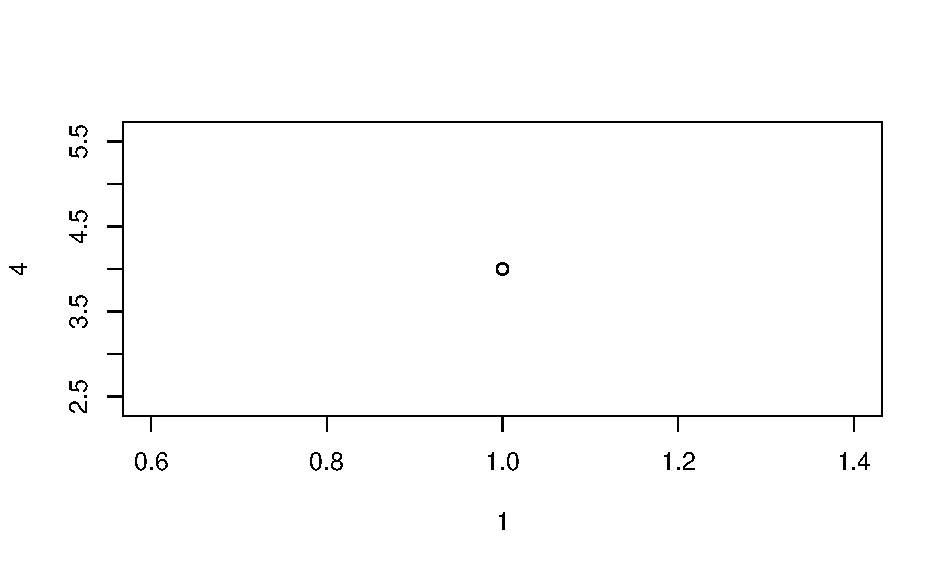
\includegraphics{03-roz3_files/figure-pdf/fig-rycina1-1.pdf}

}

\caption{\label{fig-rycina1}Moja pierwsza rycina}

\end{figure}

\begin{figure}[t]

{\centering \includegraphics[width=1\textwidth,height=3.125in]{figures/rcookies.png}

}

\caption{\label{fig-rycina2}Moja druga rycina}

\end{figure}

\bookmarksetup{startatroot}

\hypertarget{sec-metody}{%
\chapter{Metody}\label{sec-metody}}

Rozdział \textbf{Metody} zawiera opis użytych metod (np. statystycznych
czy geostatystycznych) oraz technologii (np. pakiety R). Opis każdej z
metod czy technologi powinien być zwarty i zawierać tylko najważniejsze
informacje z punktu widzenia pracy dyplomowej.

Każda użyta metoda i technologia powinna być zacytowana. W przypadku
pakietów R, wystarczy wypełnić poniższy blok kodu (zwróć uwagę, że ten
blok kodu ma parametr \texttt{echo:\ false}; oznacza to, że będzie on
niewidoczny w wynikowym pliku PDF)\ldots{}

\ldots{} a następnie zacytować pakiet używając znaku \texttt{@}, po
którym podać nazwę pakietu rozpoczynającą się od prefiksu \texttt{R-}.
Przykładowe cytowanie języka R bez nawiasu to \textcite{R-base}, a
pakietu \textbf{kableExtra} w nawiasie to \autocite{R-kableExtra}.
Więcej przykładów cytowania można znaleźć na stronie
https://rmarkdown.rstudio.com/authoring\_bibliographies\_and\_citations.html\#citations.

W przypadkach, gdy cytowanie istnieje, ale nie jest pakietem R to należy
dodać je do pliku \texttt{thesis.bib} i użyć powyższej składni ze
znakiem \texttt{@}. W ostateczności, gdy dana technologia nie posiada
cytowania, należy podać jej adres internetowy.

\bookmarksetup{startatroot}

\hypertarget{sec-wyniki}{%
\chapter{Wyniki}\label{sec-wyniki}}

Część \textbf{Wyniki} może składać się z jednego lub więcej rozdziałów.
Każdy z tych rozdziałów powinien mieć tytuł adekwatny do swojej treści.

Rozdziały wynikowe powinny korzystać z wiedzy opisanej w poprzednich
rozdziałach (Rozdziały \ref{sec-lit}, \ref{sec-materialy},
\ref{sec-metody}). W przypadku prac analitycznych, ich treść powinna
przedstawiać kolejne etapy eksploracji i analizy danych. W przypadku
prac technicznych, treść tych rozdziałów powinna opisywać stworzone
narzędzia, a następnie pokazywać ich zastosowanie/a.

W przypadku prac technicznych warto pokazywać fragmenty napisanego
rozwiązania lub jego wywołania używając bloków kodu.

\begin{Shaded}
\begin{Highlighting}[]
\NormalTok{moja\_funkcja }\OtherTok{=} \ControlFlowTok{function}\NormalTok{(x)\{}
  \FunctionTok{cat}\NormalTok{(x, }\StringTok{"rządzi!"}\NormalTok{)}
\NormalTok{\}}
\FunctionTok{moja\_funkcja}\NormalTok{(}\StringTok{"Autor tej pracy"}\NormalTok{)}
\end{Highlighting}
\end{Shaded}

\begin{verbatim}
Autor tej pracy rządzi!
\end{verbatim}

\bookmarksetup{startatroot}

\hypertarget{podsumowanie}{%
\chapter{Podsumowanie}\label{podsumowanie}}

Podsumowanie pracy jest w pewnym sensie znacznie rozbudowanym
abstraktem. Należy wyliczyć i opisać osiągnięcia uzyskane w pracy
dyplomowej. Tutaj jednak (w przeciwieństwie do np. rozdziału
\ref{sec-wprowadzenie}) należy przechodzić od szczegółu do ogółu - co
zostało stworzone/określone, jak zostało to zrobione, jakie ma to
konsekwencje, itd.

Ten rozdział powinien też zawierać opis kwestii, których nie udało się
rozwiązać w pracy dyplomowej (i dlaczego się nie udało) oraz pomysły na
przyszłe ulepszenie uzyskanych wyników lub dalsze badania.

\printbibliography[heading=bibintoc, title=Bibliografia]

\end{document}
